\section{Diagrammi di sequenza}
\label{diagrammi_seq}

Di seguito sono riportati i diagrammi di sequenza delle operazioni principali di \project{}.

\subsection{Creazione di un nuovo Subject}
\label{creazione_subject}
Il diagramma seguente, descrive la sequenza di operazioni che vengono effettuate quando si procede all'inserimento di un nuovo Subject\g{}. Esso pone enfasi sulle operazioni di creazione delle varie viste necessarie, tralasciando, per agevolare la lettura, le interazioni con la base di dati.
 La sequenza delle operazioni viene scatenata dall'utente quando seleziona, dalla finestra principale di \project{} (\textit{WelcomePage}), il comando \textit{New Subject}, tramite l'apposito pulsante. Vengono successivamente effettuate le seguenti operazioni:
\begin{enumerate}
	\item Viene emesso il signal\g{} \textit{CreateNewSubject} del \textit{WelcomeController};
	\item Il \textit{WelcomeController} richiama lo slot\g{} \textit{SlotNewSubject} del \textit{MainWindowController};
	\item Il \textit{MainWindowController} crea una nuova istanza della vista \textit{NewSubjectView} che permette all'utente di interagire col sistema per inserire il Subject\g{}. In seguito \textit{MainWindowController} crea un'istanza di \textit{NewSubjectController};
	\item \textit{MainWindowController} invoca il proprio metodo \textit{RegisterToSystem}, il quale sostituisce la vista corrente (\textit{WelcomePage}) con la nuova vista \textit{NewSubjectView}, cancellandola. In seguito registra anche il nuovo controller \textit{NewSubjectController} invocando il metodo \textit{addController} di \textit{ControlManager}, cancellando anche il controller relativo alla finestra principale;
\end{enumerate}
L'utente a questo punto visualizza la vista che permette l'inserimento delle informazioni del \subject{}, quali: \textit{Nome}, \textit{Tipo}, \textit{Immagine/Video} e \textit{Maschera}. L'aggiunta dei file relativi all'immagine e alla maschera prevede le seguenti informazioni:
\begin{enumerate}
	\item Emissione del signal\g{} \textit{addImage/addMask}, raccolto dal \textit{NewSubjectController} che procede lanciando lo slot\g{} \textit{slotAddImage/slotAddMask}; quest'ultimo crea una finestra di dialogo che permette all'utente di selezionare il file relativo all'immagine;
	\item Dopo aver caricato il file, il controller invocherà il metodo \textit{setImagePath/setMaskPath}, indicando il percorso del file selezionato.
\end{enumerate}
Una volta inserite le informazioni sul \subject{}, l'utente potrà salvare il subject\g{} premendo il pulsante \textit{Save}. La pressione del pulsate provoca le seguenti operazioni:
\begin{enumerate}
	\item Emmissione del signal\g{} \textit{saveObject}, raccolto dal \textit{NewSubjectController} che procede lanciando lo slot\g{} \textit{slotSaveSubject}, il quale salva il Subject\g{} appena creato.
\end{enumerate}

Al fine di agevolare la lettura del diagramma sono state omesse le operazioni di aggiornamento della \textit{StatusBar} di \textit{MainWindow}.

\pagebreak
\begin{figure}[!h]
\centering
			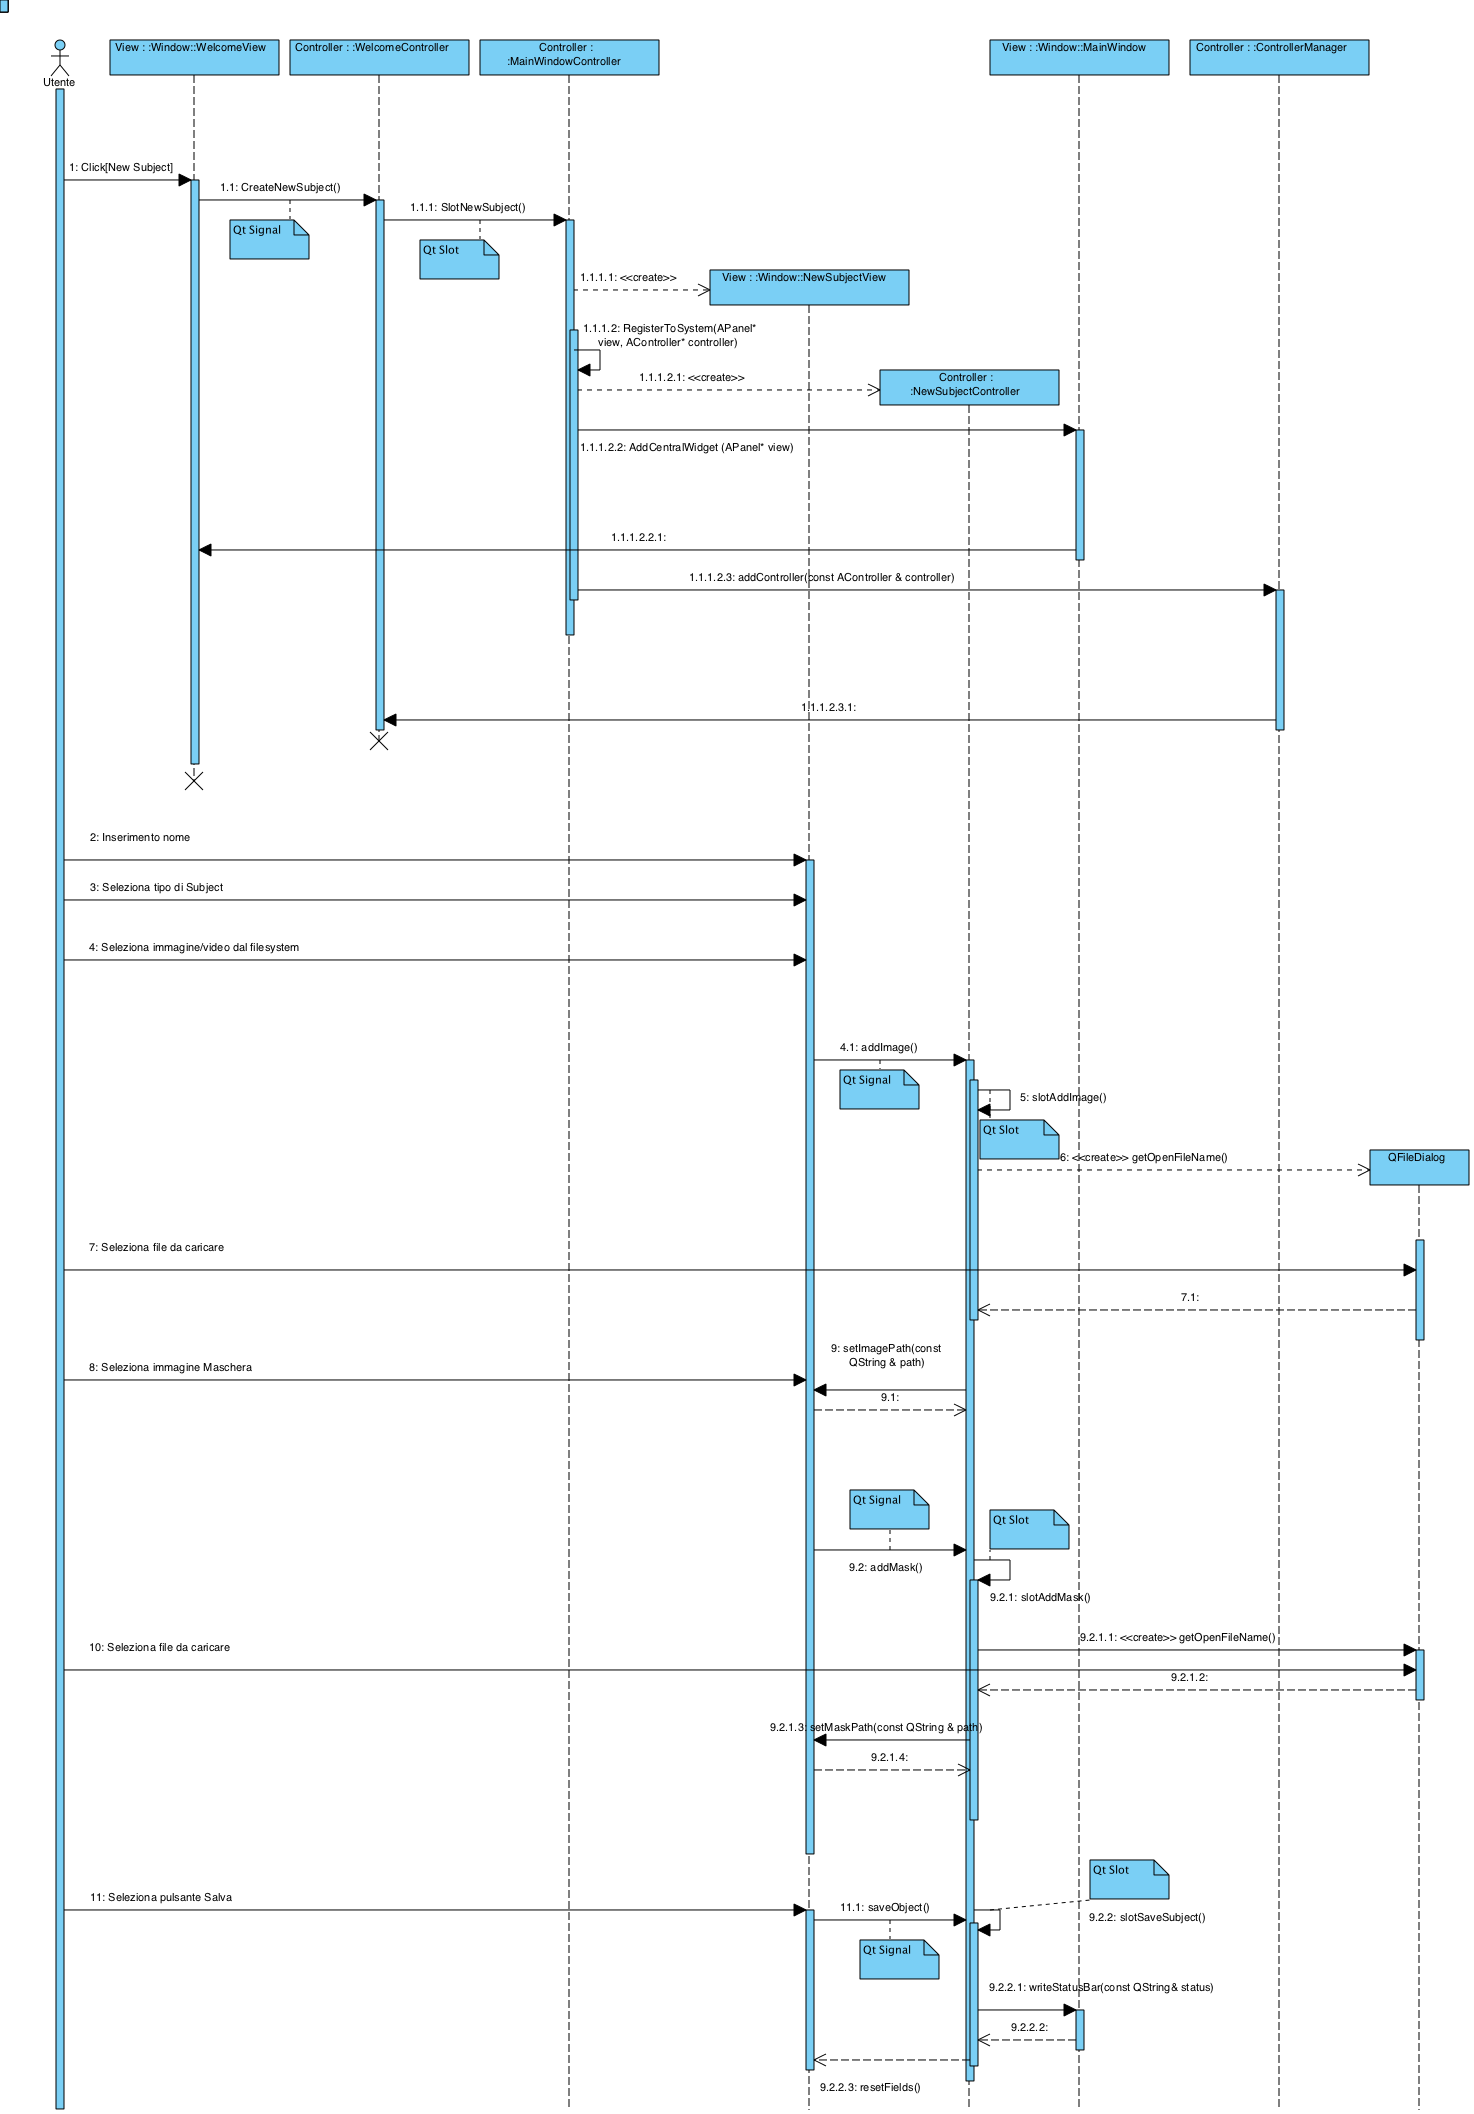
\includegraphics[width=1.12\linewidth]{./Content/Immagini/Creazione_subject.png}
			\caption{Diagramma di sequenza: creazione Subject}
			\label{creazione_subject_img}
\end{figure}
\pagebreak

\subsection{Creazione di un nuovo Protocol}
Il seguente diagramma pone enfasi sulle interazioni tra vista, controller e base di dati. La situazione descritta presuppone che l'utente si trovi nella vista di creazione di un Protocol\g{}, visto che queste sono descritte nel diagramma precedente.
L'utente interagisce con la vista inserendo il \textit{Nome} e il \textit{Tipo} del Protocol\g{}. Esso può inoltre aggiungere una o più Feature\g{}, premendo il pulsante \textit{AddFeature}. In seguito alla pressione del pulsante, vengono effettuate le seguenti operazioni:
\begin{enumerate}
	\item \textit{NewProtocolView} emette il signal\g{} \textit{addFeatureClicked}, raccolto da \textit{NewProtocolController};
	\item Il controller reagisce invocando lo slot\g{} \textit{slotAddFeatureClicked}, che interagisce con \textit{FeatCreator} per recuperare la lista delle Feature\g{} presenti (in questo caso del primo ordine), con i relativi parametri.
\end{enumerate}
A questo punto l'utente interagisce con una finestra di dialogo, che gli permette di selezionare la Feature\g{} da aggiungere e di settare i vari parametri. In seguito alla pressione del pulsante \textit{Ok}, vengono scatenate le seguenti operazioni:
\begin{enumerate}
	\item Emissione del signal \textit{Ok} da parte del dialogo \textit{FeatureParams}, che ritorna la lista dei parametri al \textit{NewProtocolController};
	\item Il controller reagisce invocando lo slot\g{} \textit{slotOk}, recuperando la Feature\g{} da aggiungere. In seguito aggiunge la Feature\g{} al \textit{NewProtocolFeatureTableModel} e distrugge la vista del dialogo.
\end{enumerate}
L'utente può aggiungere una o più Feature{}; verranno quindi ripetute le operazioni precedenti, finché l'utente non seleziona il pulsante \textit{Save}. In seguito vengono eseguite le seguenti operazioni:
\begin{enumerate}
	\item Viene emesso il signal\g{} \textit{saveObject}, raccolto dal \textit{NewProtocolController};
	\item Il controller reagisce invocando lo slot\g{} \textit{slotSaveProtocol}, che recupera dalla vista \textit{NewProtocolView} le informazioni sul \textit{Nome}, il \textit{Tipo} e le \textit{Feature} che compongono il Protocol\g{} da salvare;
	\item Il controller in seguito crea un oggetto \textit{ProtocolDAO}, che consente al sistema di salvare il Protocol\g{} sulla base di dati, tramite il metodo \textit{createProtocol};
	\item Il controller poi si preoccupa di reimpostare le varie i campi dati delle \textit{form} di inserimento, consentendo la successiva creazione di un nuovo Protocol\g{};
	\item Il controller infine invoca il metodo \textit{writeStatusBar} della \textit{MainWindow}, che informerà l'utente dell'avvenuto inserimento.
\end{enumerate}

\pagebreak
\begin{figure}[!h]
\centering
			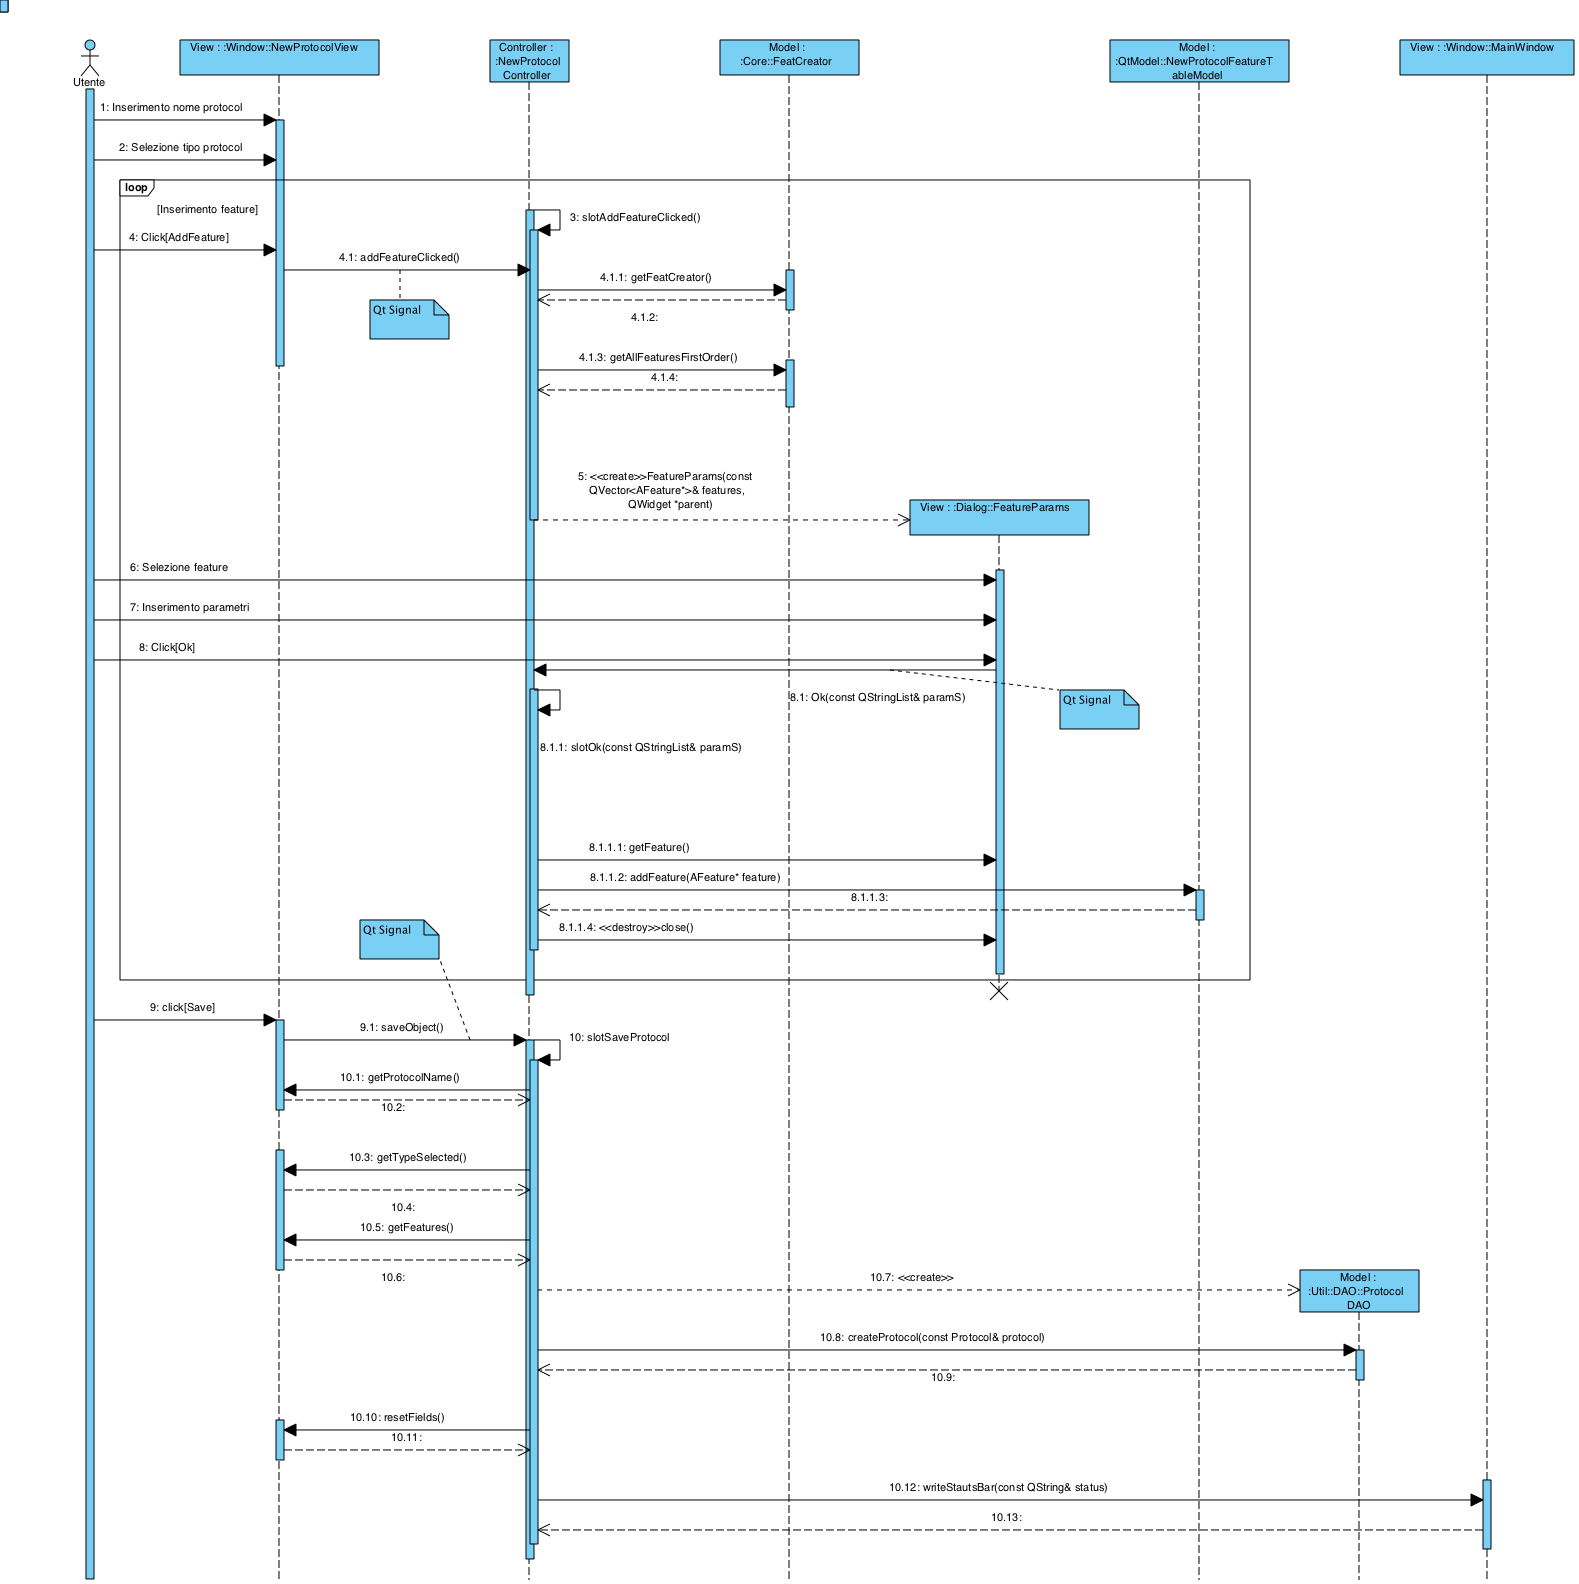
\includegraphics[width=1.12\linewidth]{./Content/Immagini/Creazione_protocol.png}
			\caption{Diagramma di sequenza: creazione Protocol}
			\label{creazione_protocol_img}
\end{figure}
\pagebreak

\subsection{Avvio di un'analisi}
\label{avvio_analisi}
Il diagramma seguente descrive la sequenza di operazioni che vengono effettuate quando si procede all'avvio di un'analisi.
La situazione descritta presuppone che l'utente si trovi nella vista di avvio analisi. L'utente potrà selezionare il \textit{Dataset} sul quale effettuare l'analisi, un insieme di \subject{}, le Feature\g{} di cui vogliamo esportare i risultati e quelle di cui vogliamo visualizzare l'anteprima durante l'analisi.
Dovrà inoltre selezionare la cartella di destinazione dei risultati; questo comporterà le seguenti operazioni:
\begin{enumerate}
	\item Emissione di un signal\g{} da parte della \textit{AnalysisView}, raccolto dall'\textit{AnalysisController};
	\item Il controller reagisce invocando lo slot\g{} \textit{slotSelectResultsFolder}, il quale crea una nuova finestra di dialogo dal quale l'utente può specificare la cartella di destinazione;
	\item In seguito il controller invoca il metodo \textit{setDestinationFolder} della vista il quale imposta il campo in cui viene visualizzato il path di esportazione selezionato.
\end{enumerate}
A questo punto l'utente può avviare l'analisi premendo il pulsante \textit{Start Analysis}. Questo comporta le seguenti operazioni:
\begin{enumerate}
	\item Emissione del signal \textit{startAnalysis}, raccolto dall'\textit{AnalysisController};
	\item Il controller reagisce invocando lo slot\g{} \textit{slotStartAnalysis}.
\end{enumerate}

\begin{figure}[!h]
\centering
	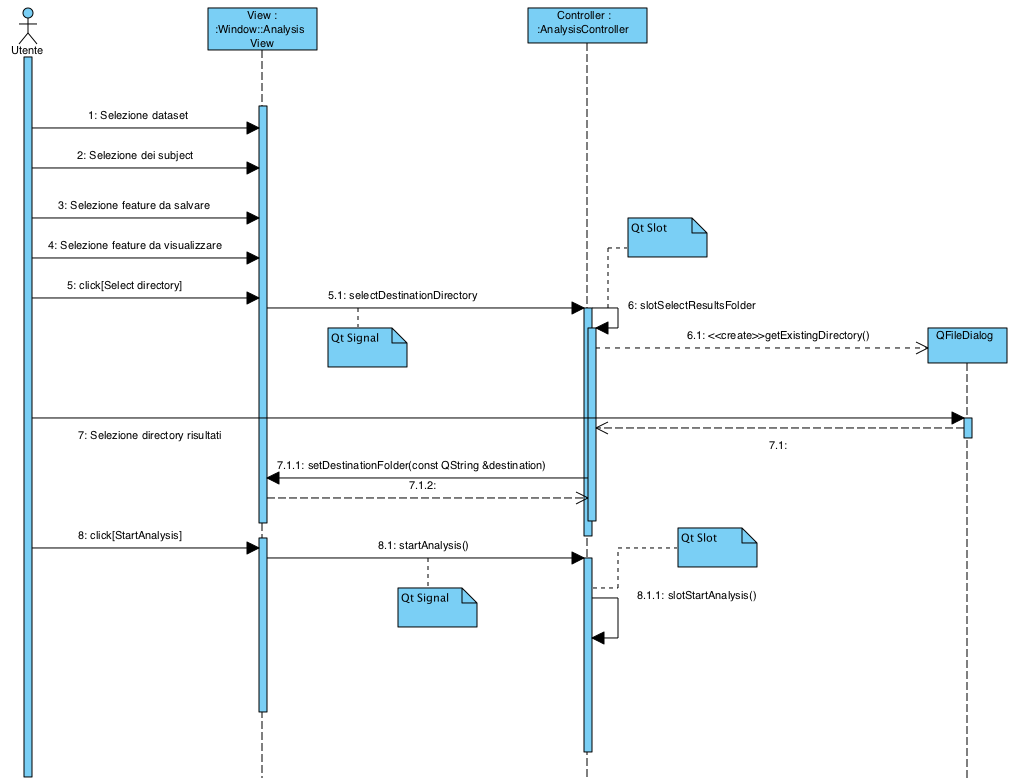
\includegraphics[width=\linewidth]{./Content/Immagini/esegui_analisi.png}
	\caption{Diagramma di sequenza: esecuzione analisi}
	\label{esegui_analisi_img}
\end{figure}
\pagebreak

\subsection{slotStartAnalysis}
\label{slotStartAnalysis}
Il diagramma seguente descrive la sequenza di operazioni che vengono effettuate quando l'utente ha cliccato il pulsante di avvio analisi.
Il controller \textit{AnalysisController} esegue queste operazioni:
\begin{enumerate}
	\item Crea una finestra di dialogo \textit{AnalysisDialog};
	\item Crea un oggetto di tipo \textit{Analysis};
	\item Invoca il metodo \textit{show} di \textit{AnalysisDialog} che mostra il dialogo dell'analisi;
	\item Invoca il metodo \textit{start} della classe \textit{Analysis}.
\end{enumerate}
A questo punto la classe \textit{Analysis} chiama il suo metodo \textit{run} che genera un ciclo, sui subject\g{} su cui viene fatta l'analisi, che esegue le seguenti operazioni:
\begin{enumerate}
	\item Emette il segnale \textit{beginSubject} che viene ricevuto dal controller \textit{AnalysisController} dal suo slot \textit{slotIncrementSubject};
	\item Lo slot chiama il metodo \textit{incrementCurrentSubject} del dialogo \textit{AnalysisDialog} che si occupa di incrementare gli indici che segnano su quale subject\g{} stiamo eseguendo l'analisi;
	\item In seguito la classe \textit{Analysis} esegue il metodo \textit{executeAnalysisOnSubject} il quale esegue l'analisi sul subject\g{} corrente;
\end{enumerate}
Dopo aver eseguito l'analisi su tutti i subject\g{} la classe \textit{Analysis} emette il segnale \textit{resultReady} che viene ricevuto dallo slot \textit{slotFinishAnalysis} del controller \textit{AnalysisController}.\\
Lo slot chiama il metodo \textit{analysisFinish} del dialogo \textit{AnalysisDialog} che imposta le informazioni del dialogo in modo da segnalare all'utente la corretta terminazione dell'analisi.\\
L'utente a questo punto può cliccare nel pulsante \lq\lq{}Ok\rq\rq{} oppure chiudere il dialogo; l'azione emette un segnale che viene ricevuto dallo slot ridefinito \textit{closeEvent} del dialogo \textit{AnalysisDialog}.\\
Questo slot emette il segnale \textit{closeOnFinish} che viene ricevuto dallo slot \textit{slotResetView} del controller \textit{AnalysisController} che reimposta la vista di avvio analisi e chiude il dialogo \textit{AnalysisDialog}.

\begin{figure}[!h]
\centering
	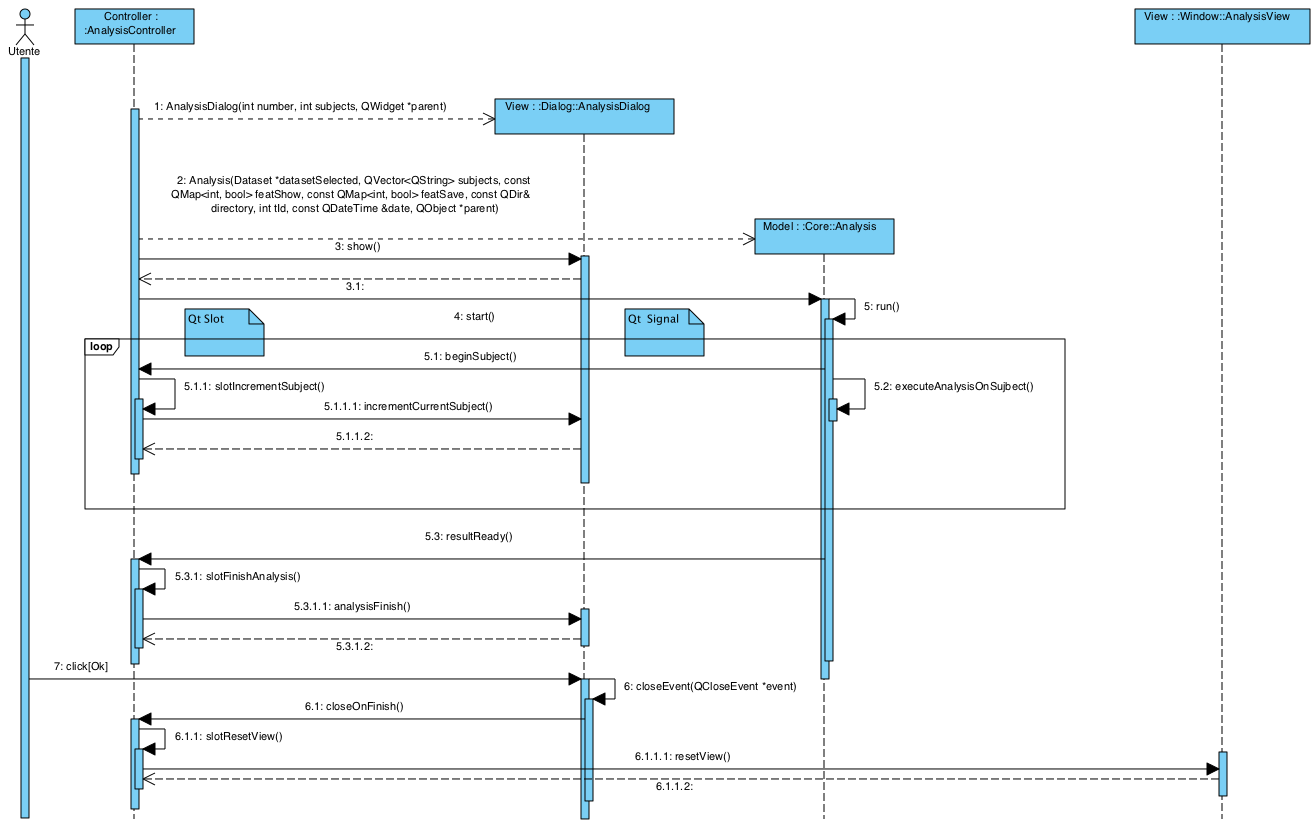
\includegraphics[width=\linewidth]{./Content/Immagini/SlotStartAnalysis.png}
	\caption{Diagramma di sequenza: slotStartAnalysis}
	\label{diag_slotStartAnalysis}
\end{figure}
\pagebreak